\documentclass[a4paper, 12pt]{article}%тип документа

%отступы
\usepackage[left=2cm,right=2cm,top=2cm,bottom=3cm,bindingoffset=0cm]{geometry}

%Русский язык
\usepackage[T2A]{fontenc} %кодировка
\usepackage[utf8]{inputenc} %кодировка исходного кода
\usepackage[english,russian]{babel} %локализация и переносы

%Вставка картинок
\usepackage{graphicx}
\graphicspath{{pictures/}}
\DeclareGraphicsExtensions{.pdf,.png,.jpg}

%Графики
\usepackage{multirow}
\usepackage{pgfplots}
\pgfplotsset{compat=1.9}

%Римские цифры
\newcommand{\RNumb}[1]{\uppercase\expandafter{\romannumeral #1\relax}}

%Математика
\usepackage{amsmath, amsfonts, amssymb, amsthm, mathtools}

%Заголовок
\author{Богданов Александр \\
	Б05-003}
\title{\textbf{Работа 5.10.1 \\ 
		Электронный парамагнитный резонанс}}

\begin{document}

\maketitle

\textbf{Цель работы:}  исследовать электронный парамагнитный резонанс в молекуле ДФПГ, определить $g$-фактор электрона,  измерить ширину ЭПР.
    
\textbf{В работе используются:} дифинилпикрилгидразил (ДФПГ),  радиоспектрометр,  осцилограф,  магнит.\\

\textbf{Теоретические положения:}\\\par

	Энергетический уровень электрона в присутствии магнитного поля с индукцией $B$ расщепляется на подуровня, расстояние между которыми равно:
		
\[ \Delta E = E_2 - E_1 = 2\mu B,  \]
где $\mu$ -- абсолютная величина проекции магнитного момента на направление поля.
	
	Между этими двумя уровнями возможны переходы.  Эти переходы могут возбуждаться внешним высокочастотным электромагнитным полем,  если оно имеет нужную частоту и нужное направление.  Резонансное значение частоты определяется:
	
\[ \hbar \omega_0 = \Delta E \]

	При переходе с нижнего на верхний уровень энергии электрон поглощает квант электромагнитной энергии,  а при обратном переходе такой же квант излучается. Возбуждение электронных резонансных переходов электромагнитным полем, имеющим частоту, определяемую формулой выше,  называется электронным парамагнитным резонансом (ЭПР).  Сигнал электронного парамагнитного резонанса наблюдается только на неспаренных электронах образца.  Наличие таких таких электронов приводит к парамагнетизму. 
	
	Связь между магнитным моментом $\mu$ электрона и его механическим моментом $\mathbf{M}$ выражается через гиромагнитное отношение $\gamma$ с помощью формулы:

\[ \mu = \gamma M \]
	
	Если магнитный момент частицы измеряется в магнитонах Бора, а механический - в $\hbar$, то их связь можно записать через $g$-фактор:
	
\[ \frac{\mu}{\mu_\text{Б}} = \frac{gM}{\hbar} \text{ или }  \frac{\mu}{\mu_\text{Б}} = gs,  \]
где $s = \frac{1}{2}$ - спин электрона.

	Выражение для $g$-фактора через определяемые экспериментально величины:
	
\[ g = \frac{\hbar \omega_0}{\mu_\text{Б} B}\]

\textbf{Экспериментальная установка:}\\\par

	\begin{figure}[h!]
	    \centering
		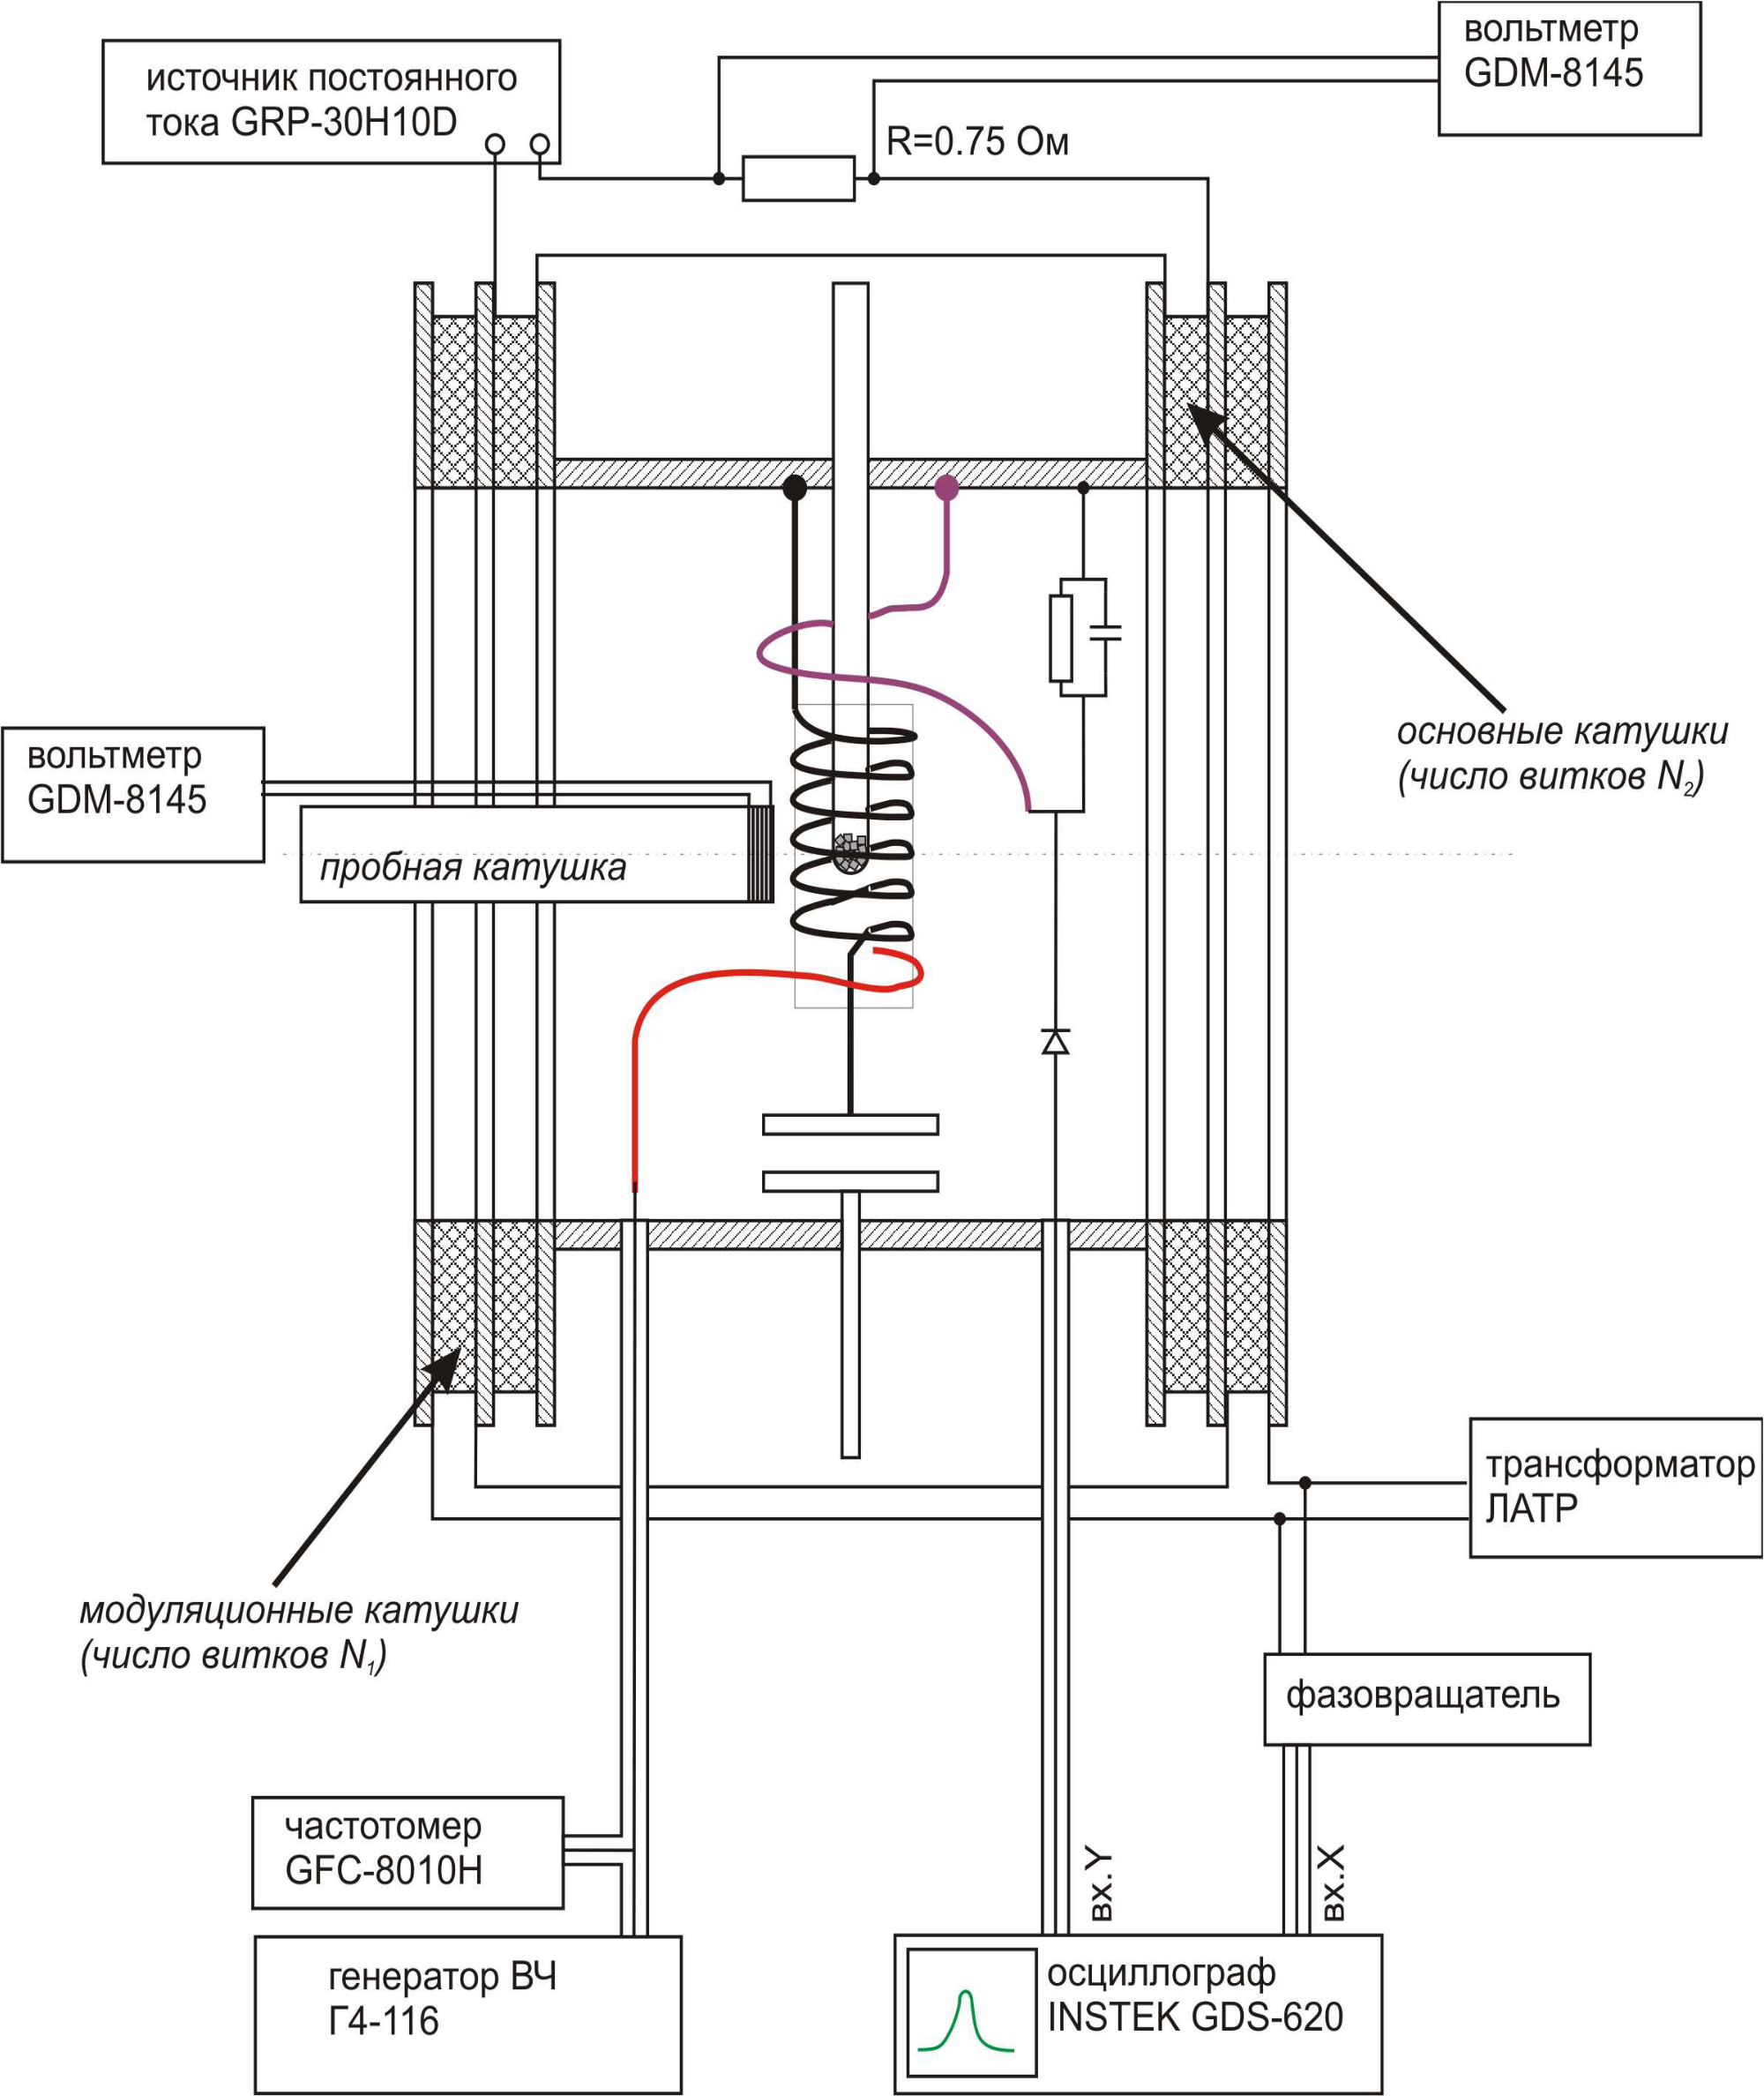
\includegraphics[scale=0.17]{Схема.png}
	\end{figure}

	Основной частью радиоспектрометра является колебательный контур,  состоящий из катушки индуктивности и плоского конденсатора.  Образец (порошок ДФПГ) в стеклянной ампуле помещается внутрь катушки.  Основное магнитное поле в образце создается с помощью двух соосно расположенных катушек,  питаемых от источника постоянного тока. 
Переменное поле небольшой амплитуды создаётся подачей на модуляционные катушки напряжения с регулируемого трансформатора.  Общая ось основных и дополнительных катушек перпендикулярна оси катушки контура. Колебания в контуре возбуждаются генератором частоты. \\

\newpage
	
\textbf{Ход работы:}\\\par

\begin{enumerate}

	\item \textbf{Получение сигнала ЭПР на свободном радикале ДФПГ и измерение $g$ - фактора электрона}
	
		\begin{enumerate}
	
		\item Настроим установку.
	
		\item Настроим генератор на резонансную частоту контура: $\omega_0 = (125 \pm 5) \text{ МГц}$.
	
		\item Параметры пробной катушки: $N = 45$,  $D = (1,45 \pm 00,1) \text{ см}$.
		
		\item Измерим частоту переменного тока: $\omega = (0,9 \pm 0,1) \text{ кГц}$.
	
		\item Показания лампового милливольтметра: $V = (9,8 \pm 1,2) \text{ мВ}$.	
		
		\item Найдем индукцию магнитного поля:
	
		\[ V = NB_0S\omega \Rightarrow B_0 = \frac{4V}{\pi N d^2 \omega}\]
	
		\[B_0 = (0,79 \pm 0,15) \text{ мТл}\]
	
		\item Посчитаем $g$ - фактор для электрона:
		
		\[ g = 1, 8 \pm 0,1\]
	
		\end{enumerate}	 
		            	    	
	\item \textbf{Определение ширины линии ЭПР}
	
		\begin{enumerate}
		
		\item Показания лампового милливольтметра: $U = (2,1 \pm 0,2) \text{ мВ}$.	
					
		\item Определим амплитуду моделирующего поля:
		
		\[B_\text{мод} = \sqrt{2} \frac{2U}{\pi^2d^2N\nu} = (1,6 \pm 0,2) \text{ Гс},\]
		где $\nu = 400 \text{Гц}$ - частота модуляции.
		
		\item Измерим полный размах модулирующего поля и ширина кривой на полувысоте:
		
		\[A_\text{полн} = (16 \pm 1) \text{ В}\]
		
		\[A_{1/2} = (0,8 \pm 0,1) \text{ В}\]
			
		\item Посчитаем ширину линии:

		\[\Delta B = \frac{A_{1/2}}{A_{\text{полн}}}B_\text{мод}\]		
		
		\[\Delta B = (0,9 \pm 0,1) \text{ Гс}\]

		\end{enumerate}	

\end{enumerate}
		
\textbf{Вывод:}\\\par

	В ходе эксперимента было исследовано явление ЭПР на молекуле ДФПГ и получены значения $g$ - фактора и полуширины линии ЭПР.  Измеренные величины получились близкими к табличным: $g_{\text{изм}} = 1, 8 \pm 0,1$ при $g_{\text{табл}} = 2$,  $\Delta B_{\text{изм}} = (0,8 \pm 0,1)\text{ Гс}$ при $\Delta B_{\text{табл}} \approx 1 \text{ Гс}$.
		
\end{document}